<<<<<<< HEAD
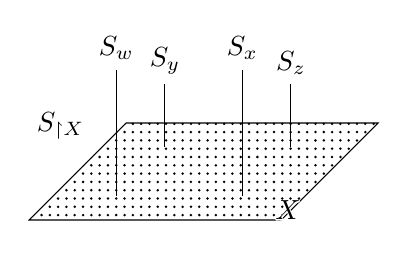
\begin{tikzpicture}[scale=0.8]
	\draw[pattern=dots] (2,0,2) -- (-2,0,2) -- (-2,0,-2) -- (2,0,-2) -- cycle node [right] {\contour{white}{$X$}};
	
	\draw (1,0,1) -- (1,2,1) node [above] {$\ms{S}_x$};
	\draw (-1,0,-1) -- (-1,1,-1) node [above] {$\ms{S}_y$};
	\draw (1,0,-1) -- (1,1,-1) node [above] {$\ms{S}_z$};
	\draw (-1,0,1) -- (-1,2,1) node [above] {$\ms{S}_w$};

	\draw (-1.5,1.5,2) node {$\ms{S}_{\upharpoonright X}$};
\end{tikzpicture}	
=======
	% Use standalone to generate PDF images
	% Recommended in slower machines and big files!
\documentclass{standalone}

	% Standard LaTeX libs
\usepackage{amssymb, mathrsfs}

	% Custom TikZ
\usepackage{tikz}
\usetikzlibrary{3d,patterns}

	% Contour for nodes
\usepackage[outline]{contour}
\contourlength{1.5pt}

	% Enable if using Overleaf to speed up compialtion times
	%\usepgfplotslibrary{external}
	%\tikzexternalize

\begin{document}
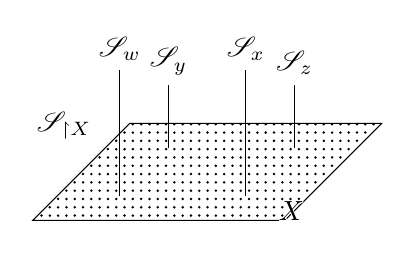
\begin{tikzpicture}[scale=0.8]
	\draw[pattern=dots] (2,0,2) -- (-2,0,2) -- (-2,0,-2) -- (2,0,-2) --
		cycle node [right] {\contour{white}{$X$}};
	
	\draw (1,0,1) -- (1,2,1) node [above] {$\mathscr{S}_x$};
	\draw (-1,0,-1) -- (-1,1,-1) node [above] {$\mathscr{S}_y$};
	\draw (1,0,-1) -- (1,1,-1) node [above] {$\mathscr{S}_z$};
	\draw (-1,0,1) -- (-1,2,1) node [above] {$\mathscr{S}_w$};

	\draw (-1.5,1.5,2) node {$\mathscr{S}_{\upharpoonright X}$};
\end{tikzpicture}	
\end{document}
>>>>>>> 1adb806 (starting to compile the examples)
